\begin{figure}[!h]
    \centering
    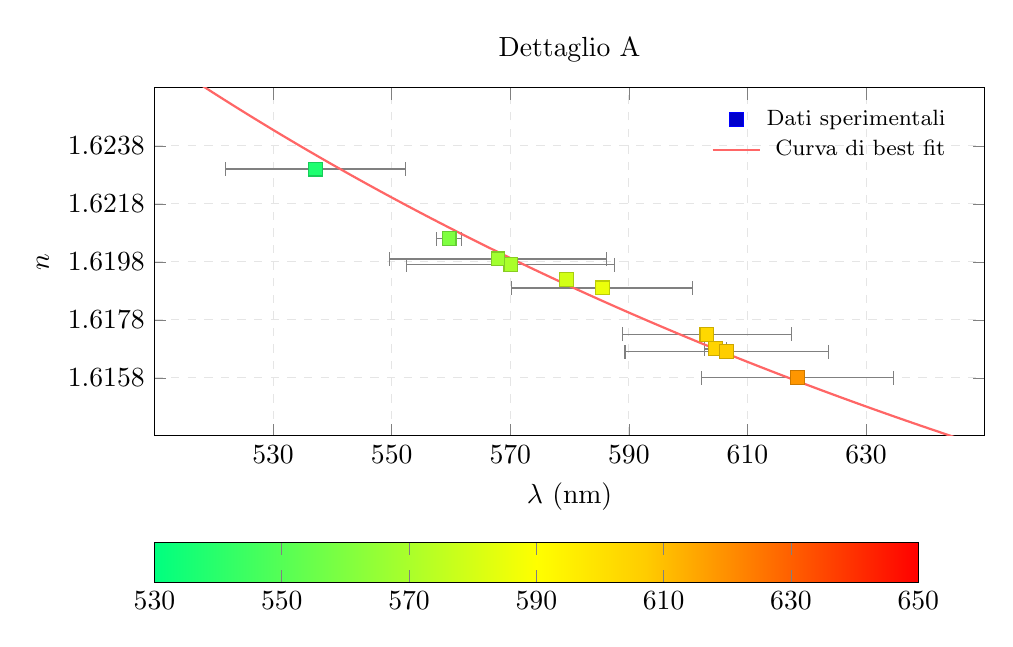
\begin{tikzpicture}
        \begin{axis}[
            title={Dettaglio A},
            width=\linewidth,
            height=6cm,
            xlabel={\(\lambda\) (nm)},
            ylabel={\(n\)},
            grid=both,
            grid style={dashed, gray!20},
            ytick={1.6158,1.6178,1.6198,1.6218,1.6238},
            yticklabels={1.6158,1.6178,1.6198,1.6218,1.6238},
            xtick={530,550,570,590,610,630},
            xticklabels={530,550,570,590,610,630},
            xmin=510, xmax=650,
            ymin=1.6138, ymax=1.6258,
            legend pos=north east,
            legend style={
                draw=none,
                fill=none,
                text opacity=1,
                font=\footnotesize,
                cells={anchor=east}
            },
            colormap={visiblespectrum}{
                rgb(510)=(0,1,0.5)   % green
                rgb(580)=(1,1,0)     % yellow
                rgb(600)=(1,0.8,0)   % orange
                rgb(650)=(1,0,0)     % red
            },
            point meta min=530,
            point meta max=650
            ]

            % Dati principali con colori dello spettro
            \addplot+ [
            scatter,
            only marks,
            mark=square*,
            scatter src=x,
            mark size=2.5,
            visualization depends on={\thisrow{yerr}\as\perror},
            visualization depends on={\thisrow{xerr}\as\xerror},
            error bars/.cd,
            x dir=both, x explicit,
            y dir=both, y explicit,
            error bar style={line width=0.5pt, solid, black!50}
            ] table [
            x=x,
            y=y,
            x error=xerr,
            y error=yerr,
            ] {
                y     yerr   x       xerr
                1.6168  0.0002  604.59  1.91
                1.6192  0.0002  579.42  1.10
                1.6206  0.0002  559.67  2.05
                1.6158  0.0002  618.41  16.20
                1.6167  0.0002  606.50  17.16
                1.6173  0.0002  603.16  14.30
                1.6189  0.0002  585.51  15.27
                1.6197  0.0002  570.11  17.54
                1.6199  0.0002  567.93  18.37
                1.6230  0.0002  537.14  15.16
            };
            \addlegendentry{Dati sperimentali}

            \addplot[
            red!60,
            thick,
            domain=340:750,
            samples=200
            ] {
                1.591703 + 9.171e3/x^2
            };
            \addlegendentry{Curva di best fit}

            % Barra dei colori con spettro visibile
            \pgfplotsset{
                colorbar horizontal,
                colorbar style={
                    xtick={530,550,570,590,610,630,650},
                    width=0.8\linewidth,
                    xlabel style={yshift=-0.5cm},
                    colormap name=visiblespectrum
                }
            }
        \end{axis}
    \end{tikzpicture}
    \caption{Ingrandimento sul raggruppamento di misure con \(\lambda > 530\)nm. I punti mantengono la colorazione secondo lo spettro visibile come nella figura principale.}
\end{figure}

